\documentclass{article}
\usepackage[T2A]{fontenc}
\usepackage{epigraph}
\usepackage[english, russian]{babel} % языковой пакет
\usepackage{amsmath,amsfonts,amssymb} %математика
\usepackage{mathtools}
\usepackage[oglav,spisok,boldsect,eqwhole,figwhole,hyperref,hyperprint,remarks,greekit]{../../style/fn2kursstyle}
\usepackage[utf8]{inputenc}
\usepackage[]{tkz-euclide}
\usepackage{algpseudocode}
\usepackage{pgfplots}
\usepackage{tikz-3dplot}
\usepackage[oglav,spisok,boldsect,eqwhole,figwhole,hyperref,hyperprint,remarks,greekit]{./style/fn2kursstyle}
\usepackage{multirow}
\usepackage{supertabular}
\usepackage{multicol}
\usepackage{tikz}
\usepackage{pgfplots}
\usepackage{float}
\usepackage{graphicx}
\pgfplotsset{compat=1.9}
\usepackage[svgnames]{pstricks}
\usepackage{pst-solides3d} 
\graphicspath{{../../style/}}
  



\newcommand{\cond}{\mathop{\mathrm{cond}}\nolimits}
\newcommand{\rank}{\mathop{\mathrm{rank}}\nolimits}
% Переопределение команды \vec, чтобы векторы печатались полужирным курсивом
\renewcommand{\vec}[1]{\text{\mathversion{bold}${#1}$}}%{\bi{#1}}
\newcommand\thh[1]{\text{\mathversion{bold}${#1}$}}
%Переопределение команды нумерации перечней: точки заменяются на скобки
\renewcommand{\labelenumi}{\theenumi)}
\newtheorem{theorem}{Теорема}
\newtheorem{define}{Определение}
\tdplotsetmaincoords{60}{115}
\pgfplotsset{compat=newest}

\title{Итерационные методы решения систем
линейных алгебраических уравнений}
\author{Н.\,О.~Акиньшин}
\group{ФН2-51Б}
\date{2024}
\supervisor{А.\,С.~Джагарян}



\begin{document}
    \maketitle
    \newpage
    \tableofcontents
    \newpage

    \section{Контрольные вопросы}
    \begin{enumerate}
        \item Почему условие $\|C\| < 1$ гарантирует сходимость итерационных методов?
        \newline
        {\bfseries Ответ.}
        Любой одношаговый итерационный метод можно записать в виде 
        \begin{equation*}
            B_{k+1}\frac{x^{k+1} - x^k}{\tau_{k+1}} + A x^k = b, \ k = 0, 1, 2,\ldots
        \end{equation*}
        Из этого вида можно прийти к следующему:
        \begin{equation}
            x^{k+1} = Cx^k + y
            \label{special form iter method}
        \end{equation}
        Подставив истинное решение $x$ в~\eqref{special form iter method},
        получим 
        \begin{equation*}
            x \equiv  Cx + y 
        \end{equation*}
        Тогда, вычитая из~\eqref{special form iter method},
        \begin{equation*}
            x^{k+1} - x = C(x^{k} - x)
        \end{equation*}
        Переходя к выражению с нормами
        \begin{equation*}
            \|x^{k+1} - x\| = \|C(x^{k} - x)\| \leqslant
           \|C\| \|x^{k} - x\| \leqslant \ldots \leqslant \|C\|^{k}\|x_0 - x\|
        \end{equation*}
        Если $\|C\| < 1$, то последовательность сходится $\{x^k\}_{k=1}^\infty$ сходится к $x$ для 
        любого $x_0$.

        
        \item Каким следует выбирать итерационный параметр $\tau$ в методе 
        простой итерации для увеличения скорости сходимости?
        Как выбрать начальное приближение $x_0$?
        \newline
        {\bfseries Ответ.}

        \item На примере системы из двух уравнений с двумя неизвестными
        дайте геометрическую интерпретацию метода метода
        Якоби, метода Зейделя, метода релаксации.
        \newline
        {\bfseries Ответ.}
        Рассмотрим метод Якоби.
        \begin{equation}
            \begin{dcases}
                a_{11}x_1^{k+1} + a_{12}x_2^k = b_1, \\
                a_{21}x_1^{k} + a_{22}x_2^{k+1} = b_2,
            \end{dcases}
            \label{system_jacoby}
        \end{equation}
        Пусть $l_1: a_{11}x_1^{k+1} + a_{12}x_2^k = b_1$, и 
        $l_2: a_{21}x_1^{k} + a_{22}x_2^{k+1} = b_2$ -- прямые, задаваемые уравнениями системы.
        Точка их пересечения и есть истинное решение системы~\eqref{system_jacoby}. 
        На рис.~\ref{jacoby_graph} видно, что с каждой итерацией точка $x^k = (x_1^k, x_2^k)$ 
        сходится к истинному решению $x$, причем каждая точка $x^k$ лежит внутри области, ограниченных прямыми.
        Причем ни одна из итеративных точек не лежит на прямых.
        \begin{figure}[H]
            \center
            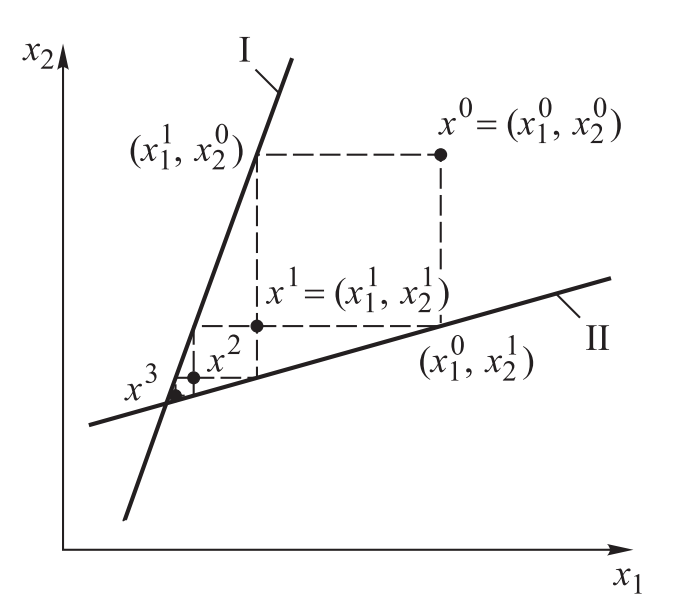
\includegraphics[width=0.5\textwidth]{jacoby_graph.png}
            \caption{Графический смысл метода Якоби}
            \label{jacoby_graph}
        \end{figure}
        Рассмотрим метод Зейделя.
        \begin{equation}
            \begin{dcases}
                a_{11}x_1^{k+1} + a_{12}x_2^k = b_1, \\
                a_{21}x_1^{k+1} + a_{22}x_2^{k+1} = b_2,
            \end{dcases}
            \label{system_seidel}
        \end{equation}
        Аналогично, принимая за прямые $l_1 = a_{11}x_1^{k+1} + a_{12}x_2^k = b_1$ и 
        $l_2 = a_{21}x_1^{k+1} + a_{22}x_2^{k+1} = b_2$ за прямые. Изобразим эти прямые на 
        рис.~\ref{seidel_graph}. Из рис.~\ref{seidel_graph} видно, что все точки лежат на прямых.
        \begin{figure}[H]
            \center
            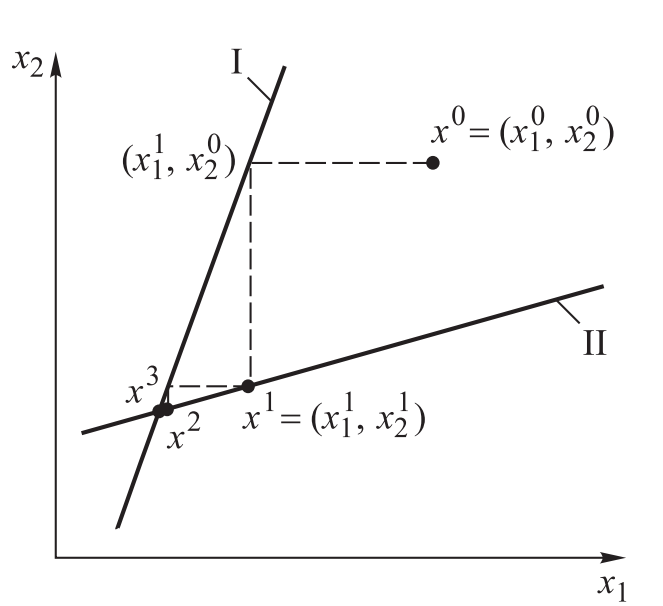
\includegraphics[width=0.5\textwidth]{seidel_graph.png}
            \caption{Графический смысл метода Зейделя}
            \label{seidel_graph}
        \end{figure}

        Рассмотрим метод релаксации. 
        \begin{equation}
            \begin{dcases}
                a_{11} (x_1^{k+1} - x_1^k) = \omega (-a_{11}x_1^k - a_{12}x_2^k +f_1), \\ 
                a_{22} (x_2^{k+1} - x_2^k) = \omega (-a_{21}x_1^k - a_{22}x_2^k +f_2)
            \end{dcases}
        \end{equation}
        Пусть $\boldsymbol{l_1} = (a_{11}, -a_{12})$ -- вектор нормали первой прямой, тогда 
        величина 
        \begin{equation*}
        |\omega (-a_{11}x_1^k - a_{12}x_2^k +f_1)| = \omega d_1 \|\boldsymbol{l_1}\|,
        \end{equation*}
        где $d_1$ -- расстояние от $(x_1^k, x_2^k)$ до первой прямой.
        \item При каких условиях сходятся метод простой итерации,
        метод Якоби, метод Зейделя и метод релаксации? Какую
        матрицу называют положительно определенной?
        \newline
        {\bfseries Ответ.}

        \item Выпишите матрицу $C$ для методов Зейделя и релаксации.
        \newline
        {\bfseries Ответ.} 
        Рассмотрим метод Зейделя.
        Будем считать, что $A = L + D + U$, где $L$ -- нижнетреугольная матрица, $D$ -- 
        диагональная матрица, $U$ -- верхнетреугольная матрица.
        Тогда метод Зейделя можно представить в каноническом виде: 
        \begin{equation*}
            (D + L)(x^{k+1} -x^k) + Ax^k = f
        \end{equation*}
        Из этого вида получаем:
        \begin{equation*}
            C = E - (D+L)^{-1}A
        \end{equation*}

        Рассмотрим метод релаксации.
        Метод релаксации можно представить в каноническом виде: 
        \begin{equation*}
            (D + L)\frac{x^{k+1} -x^k}{\omega} + Ax^k = f
        \end{equation*}
        Тогда 
        \begin{equation*}
            C = E - \omega(D+L)^{-1}A
        \end{equation*}
        \item Почему в общем случае для остановки итерационного
        процесса нельзя использовать критерий $\|x^k - x^{k+1}\| < \varepsilon$?
        \newline
        {\bfseries Ответ.}

        \item Какие еще критерии окончания итерационного процесса
        Вы можете предложить?
        \newline
        {\bfseries Ответ.}

    \end{enumerate}
    
\end{document}
